% Section 3.3 (distance) and 3.4 (surface brightness) of the Silk Nebula comment
\subsection{Distance: W26 Table~4 units and the absence of kinematic distance information}
\label{sec:distance}

W26 Sect.~3.3 derives Monte Carlo and traditional kinematic distances with the \texttt{kd} code \citep{Wenger2018} and the \citet{Reid2014} rotation curve. The footnotes to W26 Table~4 give them ``in units of 100pc'', and W26 adopts ``a fiducial distance of $\sim$160\,pc'', ``the approximate median of the six \Oiii-based kinematic distance estimates''. We tested the unit using only W26's printed values and the rotation curve it names (Section~\ref{sec:data}).

Inverting the printed \vlsr\ along the W26 Table~1 sightlines reproduces the \Oiii\ traditional distances read as kpc: we obtain 1.785 against the printed 1.79 (P1), 1.743 (1.803 from the printed \vhel) against 1.85 (P2), and 1.154 against 1.20 (P3). Comparing each printed \vlsr\ with the rotation velocity at the printed distance gives $\chi^2=0.05$ for the three \Oiii\ rows in kpc and $\chi^2=28.9$ (3 degrees of freedom, $p=2\times10^{-6}$) in units of 100\,pc (Figure~\ref{fig:distance}a); for all 15 rows the values are 15.9 ($p=0.39$) and 73.0 ($p=1\times10^{-9}$; Figure~\ref{fig:distance}c). Seven curve variants, including that of \citet{Reid2019}, give \Oiii\ distances at least 9 times the 100-pc reading. At 160\,pc, rotation produces only 1.5--1.7\,\kms\ toward P1--P3, whereas 97.5\% of the \Oiii\ velocities in the W26 Fig.~5 histogram exceed $+2.3$\,\kms, which requires $d>0.23$\,kpc on the P1 curve (Figure~\ref{fig:distance}a,b).

Two further properties of W26 Table~4 require kpc. First, a velocity width $W_V$ maps to a Monte Carlo interval of width $W_d\approx W_V/({\rm d}V/{\rm d}d)$, which other error terms only widen, so for the tabulated velocity errors $W_V/W_d$ cannot exceed the rotation gradient, 5.8--10.7\,\kms\,kpc$^{-1}$ along P1--P4. Read as 100\,pc, the \Oiii\ intervals imply 37--47\,\kms\,kpc$^{-1}$, and 13 of 15 rows exceed the bound; read as kpc, all 15 lie below it (Figure~\ref{fig:distance}d). Second, the Monte Carlo lower bounds of all 12 red-line rows, 0.00--0.02, match the 0.01-kpc floor of the \texttt{kd} distance grid; read as 100\,pc they would lie below it.

The fiducial 160\,pc is 100 times the median, 1.605, of the six \Oiii\ values (1.63, 1.58, 0.98, 1.79, 1.85, 1.20). The kinematic distance implied by W26's own analysis is therefore $\sim$1.6\,kpc, and the $\sim$28\,pc extent (281\,pc at 1.605\,kpc), the $\sim$30\,pc radius, and the energy and age derived at 160\,pc (W26 Sects.~3.3 and 4.1) do not follow from the data.

\begin{figure*}
\centering
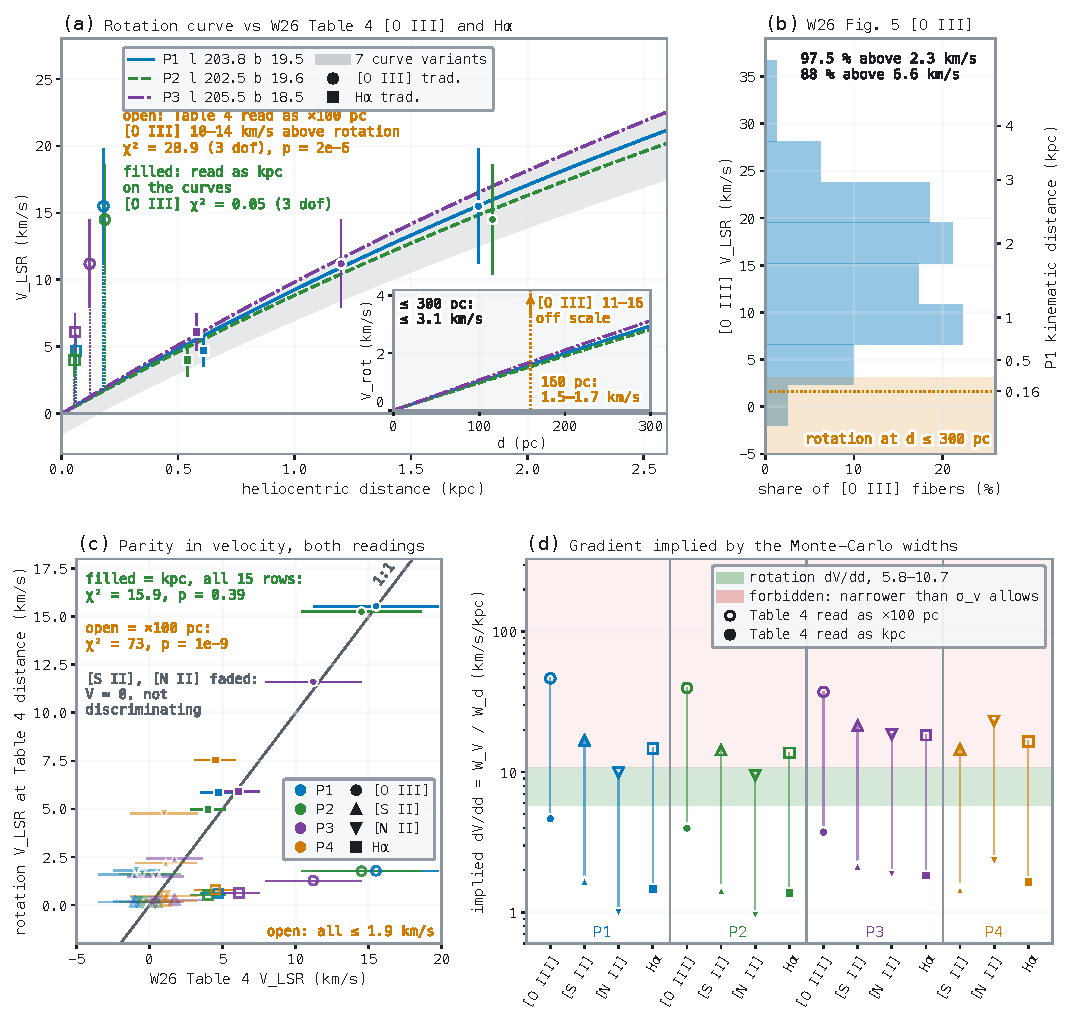
\includegraphics[width=\textwidth]{figures/dispute_distance_fig1.pdf}
\caption{W26 \citep{Wu2026} Table~4 distances read as kpc (filled symbols) and as 100\,pc (open symbols), compared with the \citet{Reid2014} rotation curve in its \texttt{kd} form \citep{Wenger2018}. (a) Rotation \vlsr\ versus distance toward P1--P3 (gray band, seven curve variants), with \Oiii\ and \Ha\ \vlsr\ $\pm\sigma_v$ at the traditional distances; inset, 0--300\,pc. (b) \Oiii\ \vlsr\ histogram digitized from W26 Fig.~5; shaded band, rotation within 300\,pc; dotted line, rotation at 160\,pc; right axis, P1 kinematic distance. (c) Rotation \vlsr\ at the printed distance versus printed \vlsr\ $\pm\sigma_v$ for all 15 rows (\Sii\ and \Nii\ faded). (d) Gradient $W_V/W_d$ implied by each Monte Carlo interval ($W_d$, printed width; $W_V$, 68.3\% velocity width for the tabulated $\sigma_v$); lower band, rotation gradient (curve variants and the Oort term of \citealt{Bovy2017}); upper shading, intervals narrower than $\sigma_v$ allows.}
\label{fig:distance}
\end{figure*}

W26 Sect.~3.3 notes that the nebula lies near the boundary of the anticenter region excluded from kinematic analysis; 8.1$^\circ$ of the 16.9$^\circ$ spine lies within the $160^\circ<\ell<200^\circ$ band masked by \citet{Wenger2018} (Figure~\ref{fig:kinematic}a). In this direction the rotational signal is comparable to typical peculiar velocities: toward P1--P4 the mean rotation gradient over 0--2\,kpc is 7.6--9.1\,\kms\,kpc$^{-1}$, so peculiar velocities of 5--10\,\kms\ \citep{Stark1989,Anderson2012,Reid2019} shift the distance by 0.55--1.32\,kpc. Within 300\,pc, rotation toward P1--P4 contributes at most 3.1\,\kms, so the \vlsr\ of a nearby object is essentially its peculiar velocity. In the \citet{Redfield2008} model, the Local Interstellar Cloud (LIC) and the Gem cloud, both within 15\,pc, project to \vlsr\ $=+7.0$ and $+21.8$\,\kms\ toward P1 and would receive kinematic distances of 0.74 and 2.70\,kpc (Figure~\ref{fig:kinematic}b).

The \texttt{kd} Monte Carlo behind W26 Table~4 contains no peculiar-velocity term \citep{Wenger2018}. With a peculiar-velocity dispersion $\sigma_{\rm pec}=10$\,\kms, the 16--84\% posterior interval for the W26 P1 \Oiii\ velocity widens from 1.28--2.51 to 0.94--3.85\,kpc, and that for the corrected \vlsr\ $=+1.2\pm1.0$\,\kms\ (Section~\ref{sec:oiii}) from 0.06--0.23 to 0.26--1.90\,kpc (Figure~\ref{fig:kinematic}c,d). The posterior is thus set by the adopted $\sigma_{\rm pec}$, not by the measurement, and the W26 data do not constrain the distance; Section~\ref{sec:location} discusses non-kinematic constraints.

\begin{figure*}
\centering
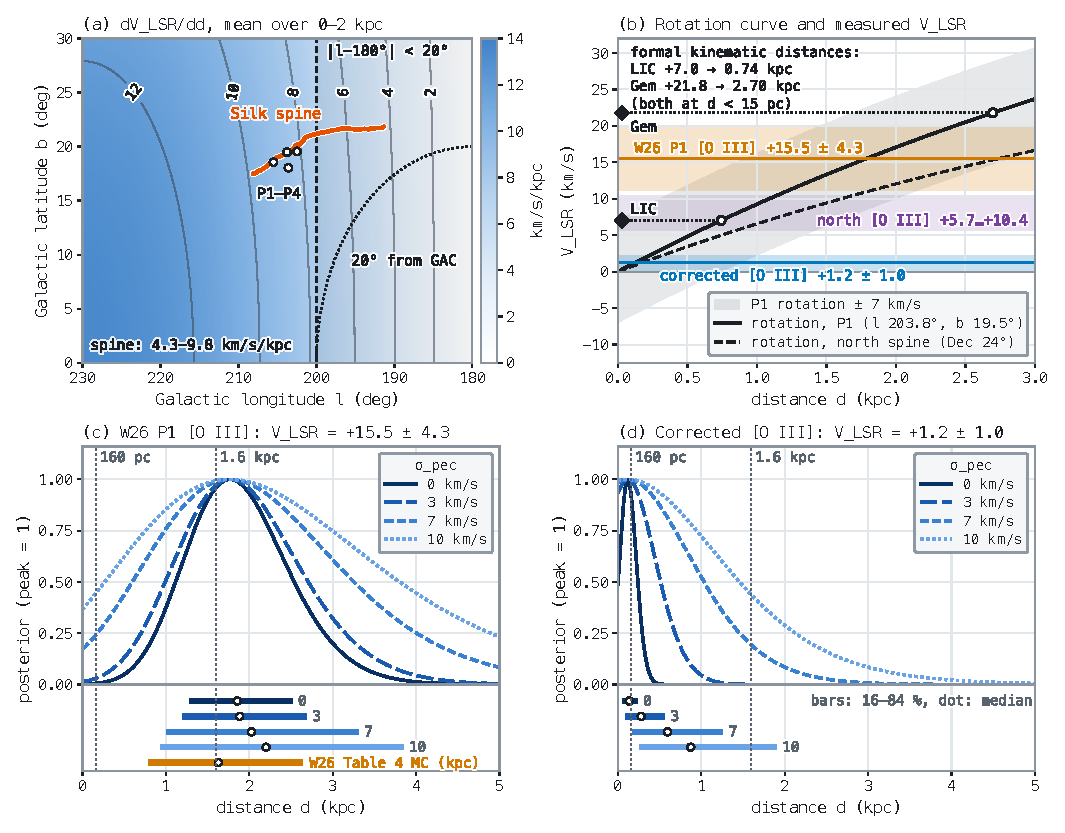
\includegraphics[width=\textwidth]{figures/dispute_kinematic_fig2.pdf}
\caption{Kinematic distances toward the Silk Nebula for the rotation curve of Figure~\ref{fig:distance}. (a) Mean rotation gradient ${\rm d}V_{\rm LSR}/{\rm d}d$ over 0--2\,kpc (contours; \kms\,kpc$^{-1}$), with the \Oiii\ spine and P1--P4 (dots); dashed line, edge of the $160^\circ<\ell<200^\circ$ band masked by \citet{Wenger2018}; dotted curve, $20^\circ$ from the Galactic anticenter (GAC). (b) Rotation \vlsr\ toward P1 (solid; gray band, $\pm7$\,\kms) and toward the spine at Dec $+24^\circ$ (dashed); horizontal bands, \Oiii\ \vlsr\ of W26 \citep{Wu2026} for P1, the corrected value (Section~\ref{sec:oiii}) and the northern DESI range (Section~\ref{sec:spectrum}); diamonds, the LIC and Gem clouds \citep{Redfield2008}; open circles, their formal kinematic distances. (c, d) Peak-normalized posteriors $P(d\,|\,V_{\rm LSR})$ toward P1 for \vlsr\ $=+15.5\pm4.3$ and $+1.2\pm1.0$\,\kms\ and $\sigma_{\rm pec}=0$, 3, 7 and 10\,\kms\ (flat prior on 0--6\,kpc; curve parameters marginalized); bars, 16--84\% intervals with medians; lowest bar in (c), W26 Table~4 Monte Carlo interval read as kpc.}
\label{fig:kinematic}
\end{figure*}

\subsection{Surface brightness}
\label{sec:brightness}

W26 Table~3 lists \Oiii-band surface brightnesses of 23.60, 23.87 and 23.85\,mag\,arcsec$^{-2}$ for P1--P3, which W26 Sect.~4.1 converts to ``$\sim$10--13 Rayleigh'', ``well above'' the 0.5--5\,R detection limit of the \citet{Fesen2024} images. The conversion is correct: an AB magnitude \citep{Oke1983} in a 60-\AA\ band containing only \Oiii~$\lambda$5007 gives 12.75, 9.94 and 10.12\,R.

Independent data are lower (Figure~\ref{fig:brightness}b). DESI DR1 spectra \citep{DESI2026} give a southern-ridge median of 1.62\,R ($\approx$20\% calibration uncertainty; Appendix~\ref{sec:appendix-desi}); SDSS sky fibers \citep{Abdurrouf2022,SDSS2026} average 1.49, 1.78 and 1.87\,R within 0.3$^\circ$ of P1--P3; SDSS imaging sky levels \citep{Almeida2023} give $2.31\pm0.38$\,R on 17$'$ scales; and NSNS maps \citep{Ziegenbalg2025} give 2.04, 2.06 and 2.18\,R. We adopt 1.4--2.5\,R. Per region, W26 Table~3 is 4.6--8.6 times higher. It exceeds even the brightest single measurements (3.65\,R in an SDSS fiber, 3.88\,R at a DESI node, 2.95--3.64\,R in NSNS $1'$ peaks) by factors of 2.6--4.3, so angular scale does not explain it.

No identified multiplicative systematic reaches the required factor of 0.12--0.22 (Figure~\ref{fig:brightness}d): the magnitude system ($\pm0.1$\,mag; \citealt{Blanton2007}), the band width (50--70\,\AA), \Oiii~$\lambda$4959 leakage and a filter in the lens aperture (generic model; field angles 0--5$^\circ$) individually give $I_{\rm true}/I_{\rm Table\,3}=0.75$--1.27, and all lowering extremes combined, with $\sim$0.3\,mag of P1 starlight, yield 5.5--5.8\,R, still 2.6--3.7 times the independent values. A common factor would also preserve the regional ranking, yet W26 Table~3 ranks P1 brightest, which W26 Sect.~3.1 attributes to starlight, and SDSS ranks it faintest.

An additive error of 7.9--11.3\,R, 6--20\% of an in-band sky of 21.1--22.0\,mag\,arcsec$^{-2}$ (Figure~\ref{fig:brightness}c), would reproduce W26 Table~3; a background or flat-field residual or unequal starlight between source and background apertures could supply it, but the published information does not show which.

For a shock-excited filament, as W26 proposes, published shock models make 10--13\,R inconsistent with the far ultraviolet. GALEX FUV follows the southern filament at $92\pm10$\,CU per NSNS rayleigh (Section~\ref{sec:counterparts}). W26 Table~3 would make this 15--20\,CU\,R$^{-1}$, 2.9--3.8 times below the 57\,CU\,R$^{-1}$ non-resonant FUV floor of the incomplete shocks of \citet{Raymond1988} at $E(B-V)=0.03$ \citep{Schlegel1998}, the lowest among tabulated shock models \citep{Raymond1979,Cox1985,Dopita1996}.

At 1.4--2.5\,R the filament lies within the 0.5--5\,R range that W26 quotes for \citet{Fesen2024}, and its detection by \citet{Fesen2026} does not require a bright filament.

\begin{figure*}
\centering
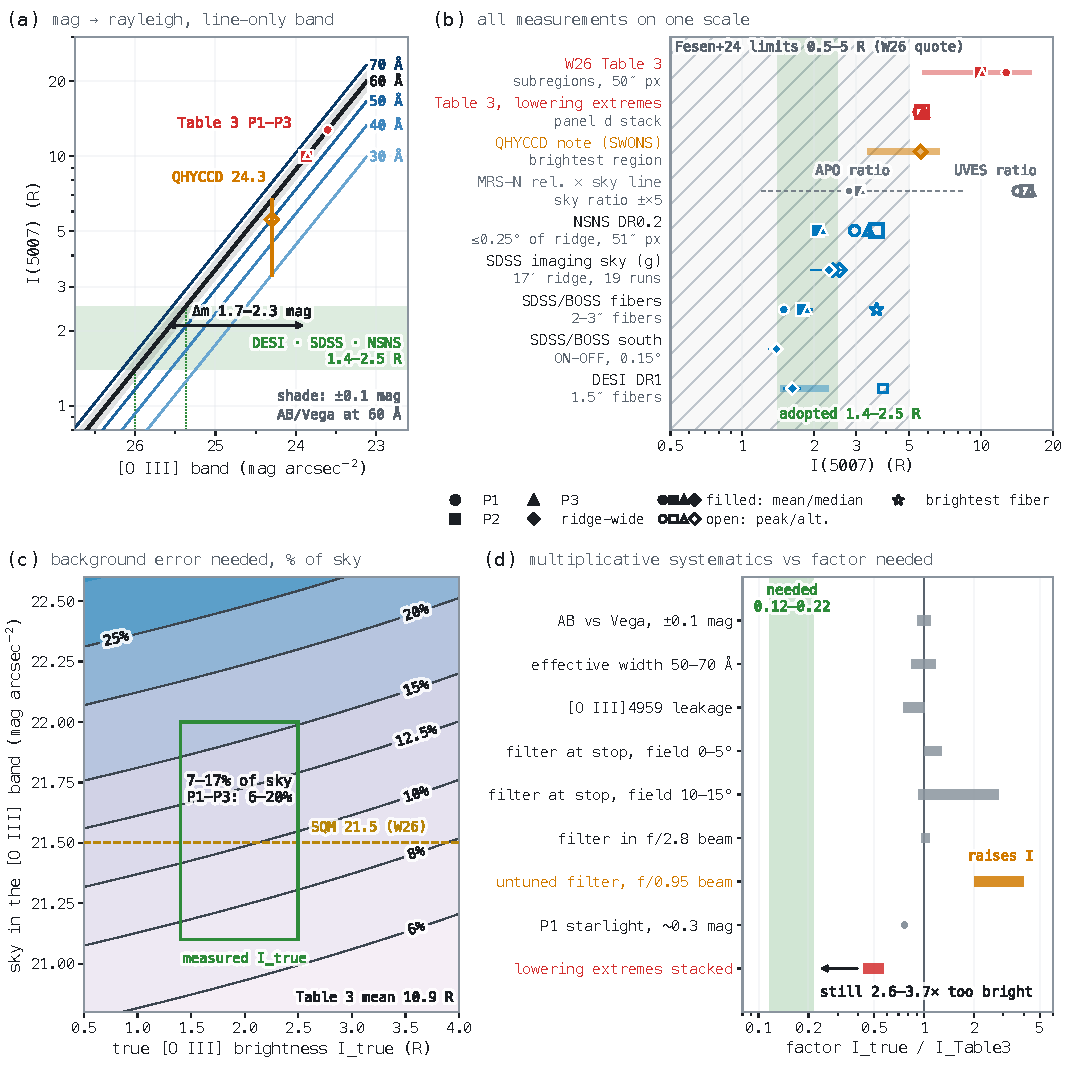
\includegraphics[width=\textwidth]{figures/dispute_brightness_5.pdf}
\caption{\Oiii~$\lambda$5007 surface brightness: W26 \citep{Wu2026} Table~3 and independent data. (a) Conversion of \Oiii-band AB surface brightness to $I(5007)$ for 30--70\,\AA\ line-only bands, with W26 Table~3, the 24.3\,mag\,arcsec$^{-2}$ reported by \citet{QHYCCD2024} for the brightest region (bar, 30--60\,\AA) and the adopted range (band). (b) Measurements by method and angular scale: W26 Table~3 (bar, conversion variants) and its combined lowering extremes; QHYCCD; MRS-N relative intensities scaled by sky-line ratios from SDSS/BOSS at Apache Point Observatory (APO; dashed, 16--84\%) or from the VLT/UVES sky atlas \citep{Hanuschik2003}; and NSNS, SDSS and DESI data \citep{Ziegenbalg2025,Almeida2023,Abdurrouf2022,SDSS2026,DESI2026}. Hatched, the 0.5--5\,R that W26 quotes for \citet{Fesen2024}; green band, adopted 1.4--2.5\,R. (c) Additive error, as a fraction of the in-band sky, that raises $I_{\rm true}$ to the W26 Table~3 mean of 10.9\,R; box, measured $I_{\rm true}$ and plausible skies; dashed line, W26 sky-quality-meter (SQM) reading. (d) Factors $I_{\rm true}/I_{\rm Table\,3}$ from single systematics (generic three-cavity 60-\AA\ filter model) and all lowering extremes combined; band, the required 0.12--0.22. The rows for field angles of 10--15$^\circ$, an f/2.8 beam and an untuned filter in an f/0.95 beam, not used in the text, give 0.93--4.0.}
\label{fig:brightness}
\end{figure*}
